De forma totalmente análoga procedemos a determinar la ganancia del SiPM en función de su voltaje operacional. Para ello, realizaremos una serie de medidas a distintos voltajes operacionales y, para cada uno de ellos, calcularemos la ganancia mediante el método expuesto anteriormente. 

Nos centraremos en el rango de voltajes entre el voltaje de ruptura, $V_{BD}= 50.97~\volt$, que es el mínimo voltaje en valor absoluto a partir del cual nos encontramos en modo Geiger y $V_{BD}+5~\volt$, que es un intervalo suficiente para compensar la ganancia en el intervalo de temperaturas que hemos medido. Realizaremos pasos de $0.2~\volt$ entre cada medida realizando un total de $25$ medidas. De nuevo, únicamente realizaremos medidas de $15000$ eventos, suficiente para obtener un espectro  suave.

Para automatizar este proceso procedemos a desarrollar una macro en ROOT que realice este ajuste. Análogamente esta macro poseerá dos partes:
\begin{itemize}
\item{} Por un lado posee un bucle en el que, en cada paso, abre el fichero correspondiente a un voltaje operacional, empezando por el mínimo ($V_{op}=V_{BD}$) realiza todo el estudio anterior y guarda ganancia y voltaje operacional con sus errores en 4 vectores respectivamente. En cada paso aumenta $0.2~\volt$ el voltaje operacional y pasa a leer el siguiente fichero. 
En este estudio, a diferencia del estudio de la temperatura, la incertidumbre en el voltaje viene dada por la precisión del electrómetro (del orden de $1~\milli\volt$) ya que el valor era perfectamente estable. Esta incertidumbre es  totalmente inapreciable tanto a nivel visual en la gráfica como a nivel de variación de la ganancia. 
Hay que tener en cuenta que el voltaje operacional posee un error relativo, definido como $\frac{\sigma_x}{x}$ muy inferior al de la temperatura, siendo estos aproximadamente $0.001\%$ y $0.8\%$ para el voltaje y la temperatura respectivamente. Es decir, las medidas tomadas en este estudio serán más precisas.

\item {} Por otro lado, partiendo de estos $4$ vectores de dimensión $25$ en nuestro caso (igual al número de ficheros que ha leído) que contienen ganancia, temperatura y sus errores de forma ordenada, realiza un ajuste lineal. El ajuste obtenido se presenta en la figura~\ref{voltaje}.

\begin{figure}[hbtp]
\centering
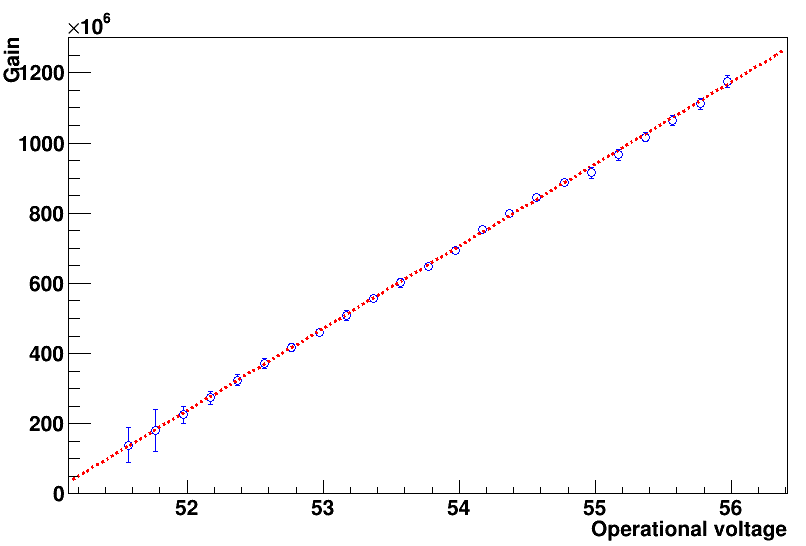
\includegraphics[scale=0.4]{Dependenciavoltaje.png}
\caption{ Ganancia frente a voltaje operacional\label{voltaje}}
\end{figure}

Podemos apreciar de nuevo, como esperábamos~\cite{tesisSiPM}, la existencia de un comportamiento  lineal casi perfecto en un intervalo de voltaje de $5~\volt$. En la gráfica podemos notar la existencia de un mayor error en las medidas de voltajes mas bajos (en valor absoluto). Esto es debido a que nos estamos acercando al voltaje de ruptura, donde el silicio entra en modo Geiger y el valor de la ganancia empieza a ser distinto de cero. Podemos achacar este mayor error a que a estos voltajes, cercanos a la frontera de cambio de comportamiento, el SiPM todavía no funciona de forma adecuada,  pues no funciona todavía en  modo Geiger. Hay que tener en cuenta además que sólo se llegó hasta el voltaje $V_{op}=51,57~\volt$  debido a que, cuando estamos a valores muy cercanos al voltaje de ruptura,  la ganancia sufre una disminución exponencial, siendo imposible realizar su medida.

De nuevo comprobamos la calidad del ajuste a partir del test $\chi^2$, obteniendo un valor de $\frac{\chi^2}{ndf}=\frac{7.963}{21}\approx 0.379$, que indica un ajuste bueno de los datos.

Podemos observar que, al contrario de lo que ocurría con la temperatura, el valor de la ganancia del SiPM aumenta a medida que aumenta el voltaje operacional. Esto es debido a que a medida que aumentamos el voltaje operacional, aumenta la diferencia de potencial en la zona desierta. De esta forma, por un lado, aumentando la zona desierta, por lo que los pares electrón-hueco dispondrán de mayor espacio para generar una avalancha mayor  y, por otro lado, estamos aplicando una mayor tensión sobre los pares electrón-hueco generados al detectar radiación que,  en consecuencia, sufrirán una mayor aceleración. Debido a ello, dispondrán de una mayor energía para producir un mayor número de pares electrón-hueco. En resumen ambos procesos contribuyen a aumentar la ganancia del SiPM.

La ecuación obtenida en este ajuste $G=cV_{op}+d$ toma los siguientes valores: 
\begin{equation}
c=(234.1 \pm 2.6) \cdot 10^6~\volt^{-1}
\label{ajustependientevoltaje}
\end{equation}
\begin{equation}
d=(-119.4 \pm 1.4) \cdot 10^8
\label{ajusteordenadavoltaje}
\end{equation}

Remarquemos de nuevo la importancia de este resultado, ya que es la parte que nos faltaba para poder calcular la compensación de la ganancia.
Además, a modo de comprobación, podemos obtener el voltaje de ruptura a partir de esta expresión, que corresponde al voltaje al cual la ganancia es cero (voltaje a partir del cual estamos en modo Geiger y la ganancia empieza a ser no nula). El voltaje calculado es: 
\begin{equation}
G=0=c \cdot V_{BD} +d \longrightarrow V_{BD}=-\frac{d}{c}=50.99 \pm 0.81~\volt
\label{ajustebdv}
\end{equation}

Vemos que este se acerca de forma extraordinaria al voltaje teórico especificado por Hamamatsu Photonics, $50.97~\volt$.
\end{itemize}